\documentclass{article}
\usepackage[utf8]{inputenc}
\usepackage[letterpaper, portrait, margin=1in]{geometry}
\usepackage{multicol}
\usepackage{amsmath}
\usepackage{amssymb}
\usepackage{enumerate}
\setlength\parindent{0pt}
\usepackage{enumerate}
\usepackage{graphicx}
\graphicspath{ {./images/} }
\usepackage{fancyhdr}
\usepackage{tcolorbox}
\hyphenchar\font=-1
\usepackage{tabularx}

\newcommand{\header}[1]{\begin{large}\noindent #1\end{large}\\\rule{\textwidth}{0.5pt}}
\newcommand{\gap}{\medskip\\}
\newcommand{\centertext}[1]{\begin{center}#1\end{center}}
\newcommand{\bfrac}[2]{\left(\frac{#1}{#2}\right)}
\newcommand{\formula}[3]{\begin{center} \begin{tcolorbox}[title = #2] $$#3$$\end{tcolorbox}\end{center}}
\newcommand{\where}{\hspace{0.5cm} \textrm{where} \hspace{0.5cm}}
\newcommand{\hgap}{\hspace{0.5cm}}
\newcommand{\pfrac}[2]{\frac{\partial #1}{\partial #2}}
\newcommand{\sheader}[1]{\underline{#1:}}
\newcommand{\doubleformula}[4]{\begin{center} \begin{tcolorbox}[title = #2] $$#3$$\\$$#4$$\end{tcolorbox}\end{center}}
\newcommand{\curly}[1]{\left\{#1\right\}}
\newcommand{\proj}[2]{{}\textrm{proj}_{#1}\left(#2\right)}

\newcommand{\ds}{\displaystyle}
\newcommand{\Arg}{\textrm{Arg}}

\newcommand{\tripleformula}[5]{\begin{center} \begin{tcolorbox}[title = #2] $$#3$$\\$$#4$$\\$$#5$$\end{tcolorbox}\end{center}}

\begin{document}
    \begin{center}
        \Large PHYS 304 Review Notes\\
        \normalsize Reese Critchlow
    \end{center}

    \header{General Forms for Solving Schrodinger Equations in Bound States}

    For a Schrodinger equation of the form:
    \begin{align*}
        -\frac{\hbar}{2m} \frac{\partial^2 \psi}{\partial x^2} + V(x) \psi = i\hbar \frac{\partial \psi}{\partial t},
    \end{align*}
    we can define a general solution for bound states to be of the 
    following form:
    \begin{align*}
        \Psi(x, t) = \sum_{n=0}^{\infty} c_n \psi_n(x) \cdot \varphi_n(t),
    \end{align*}
    where $\psi_n(x)$ is a \underline{stationery state} for the given potential
    $V(x)$, and $\varphi_n(t)$ is the time-dependance of the solution,
    given by:
    \begin{align*}
        \varphi_n(t) = e^{-iE_n t/\hbar},
    \end{align*}
    where $E_n$ is the energy corresponding to the state.
    \gap
    For the potentials that have been covered thus far in the course,
    there are two different stationery states corresponding to each 
    potential. We can also define their energies:

    \begin{multicols}{2}
        \centertext{\underline{Infinite Square Well}}
        \begin{align*}
            \psi_n &= \sqrt{\frac{2}{a}}\sin\left(\frac{n\pi}{a}x\right)\\
            E_n &= \frac{\hbar^2 k_n^2}{2m} = \frac{n^2 \pi^2 \hbar^2}{2ma^2}
        \end{align*}
        \centertext{where $k_n = \frac{n\pi}{a}$}
        \vfill\null
        \columnbreak
        \centertext{\underline{Harmonic Oscillator}}
        \begin{align*}
            \psi_n &= \left(\frac{m\omega}{\pi \hbar}\right)^{\frac{1}{4}} \frac{1}{\sqrt{2^n n!}}H_n(\xi)e^{-\xi^2/2}\\
            E_n &= \left(n + \frac{1}{2}\right) \hbar \omega
        \end{align*}
        \centertext{where $\ds \xi = \sqrt{\frac{m\omega}{\hbar}}x$}
        \vfill\null
    \end{multicols}

    The \underline{Hermite Polynomials} are also important to note:
    \begin{align*}
        H_n(\xi) = \begin{cases}
            H_0(\xi) = 1 \\
            H_1(\xi) = 2\xi\\
            H_2(\xi) = 4\xi^2-2\\
            H_3(\xi) = 8\xi^3 - 12\xi
            \end{cases}
    \end{align*}

    \sheader{Stationery States} Stationery states are states in which:
    \begin{enumerate}
        \item All expectation values are independent of time.
        \item Total energy is definite.
        \item The general solution is a linear combination of stationery
        states.
    \end{enumerate}

    \pagebreak

    It is also useful to know what the bound states look like for
    the harmonic oscillator.

    \begin{center}
        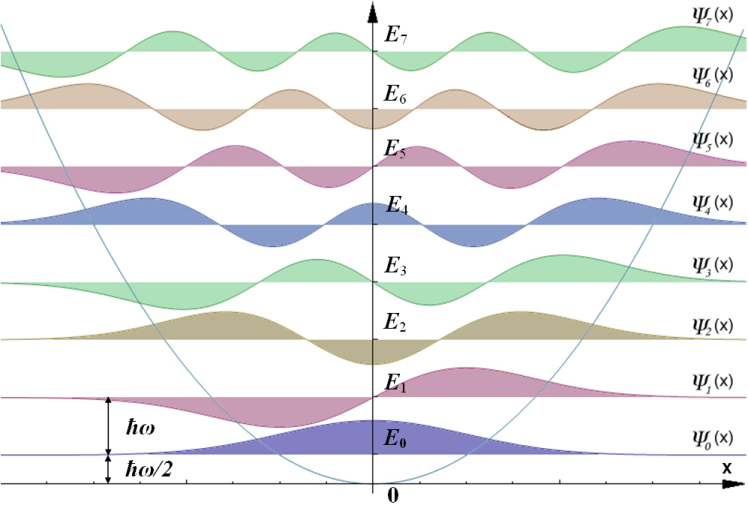
\includegraphics[scale=0.3]{harmonic-oscillator-states.png}
    \end{center}

    \header{General Forms for Solving Free Particle Problems}

    For many potentials, particles appear in \underline{scattered states},
    instead of bound states. In these cases, energies are not quantized
    and general forms are computed over integrals, not sums.
    \gap
    For the case of the \underline{free particle}, where the 
    potential is zero everywhere, one can find the solution using the
    following procedure.
    \begin{enumerate}
        \item Identify $\phi(k)$, which is the distribution of states 
        over the variable $k$, using a Fourier transform:
        \begin{align*}
            \phi(k) = \frac{1}{\sqrt{2\pi}} \int_{-\infty}^{\infty}\Psi(x, 0)e^{-ikx}dx.
        \end{align*}
        \item Transform the function out of the frequency domain using 
        another Fourier transform:
        \begin{align*}
            \Psi(x,t) = \frac{1}{\sqrt{2\pi}}\int_{-\infty}^{\infty} \psi(k) e^{i\left(kx - \frac{\hbar k^2}{2m}t\right)} dk.
        \end{align*}
    \end{enumerate}

    The distribution of states $\phi(k)$ in the general solution is known 
    as the \underline{wavepacket}. There are two velocities that are important
    in this case.
    \begin{itemize}
        \item \sheader{Phase Velocity} $\ds v_\textrm{phase} = \frac{\omega}{k} = \frac{\hbar k}{2m} = \sqrt{\frac{E}{2m}}$
        \item \sheader{Group Velocity} $\ds v_\textrm{group} = 2v_\textrm{phase} = \frac{d\omega}{dk}$
    \end{itemize}
    In all of these forms, $k$ is $k_0$, which is the fundamental 
    frequency of the group.
    \gap

    \header{Probabilities and Expectation Values}
    \sheader{Heisenberg Uncertainty Principle}
    \begin{align*}
        \sigma_x \sigma_p \geq \frac{\hbar}{2}
    \end{align*}

\end{document}